\chapter{État de l'art}

De nos jours, les technologies de réalité augmentée en vue au travers avec, ou sans, un HMD se développent très rapidement mais souffrent encore de problèmes technologiques et ergonomiques majeurs ce qui ne leur permet pas d'être utilisées dans tous les domaines d'application de la réalité augmentée\cite{li2017state}. 
Récemment, une nouvelle technologie de réalité augmentée se détachant de l'approche traditionnelle liée aux écrans, jusqu'alors inexploitée dans le domaine de l'informatique, est en train d'émerger sous le nom de réalité augmentée spatiale. Cette technologie apporte des réponses aux problèmes technologiques et ergonomiques établis et permet ainsi d'ouvrir un champ des possibles bien plus large\cite{bimber2006modern}.

\section{PapARt}
\label{sec:papart}
Comme évoqué précedemment dans l'introduction (chapitre~\ref{chap:intro}), \texttt{PapARt} ou Paper Augmented Reality Toolkit se présente sous la forme d'un kit de développement permettant de créer des applications interactives en réalité augmentée de création de dessins ou de peintures (fig~\ref{fig:papartdemo}). L'idée est de proposer une technique numérique non intrusive dont le but est de faciliter la réalisation d'une tâche complexe, telle que le dessin, tout en permettant à l'utilisateur de s'exprimer\cite{laviole2012papart}.
\begin{figure}[H]
\centering
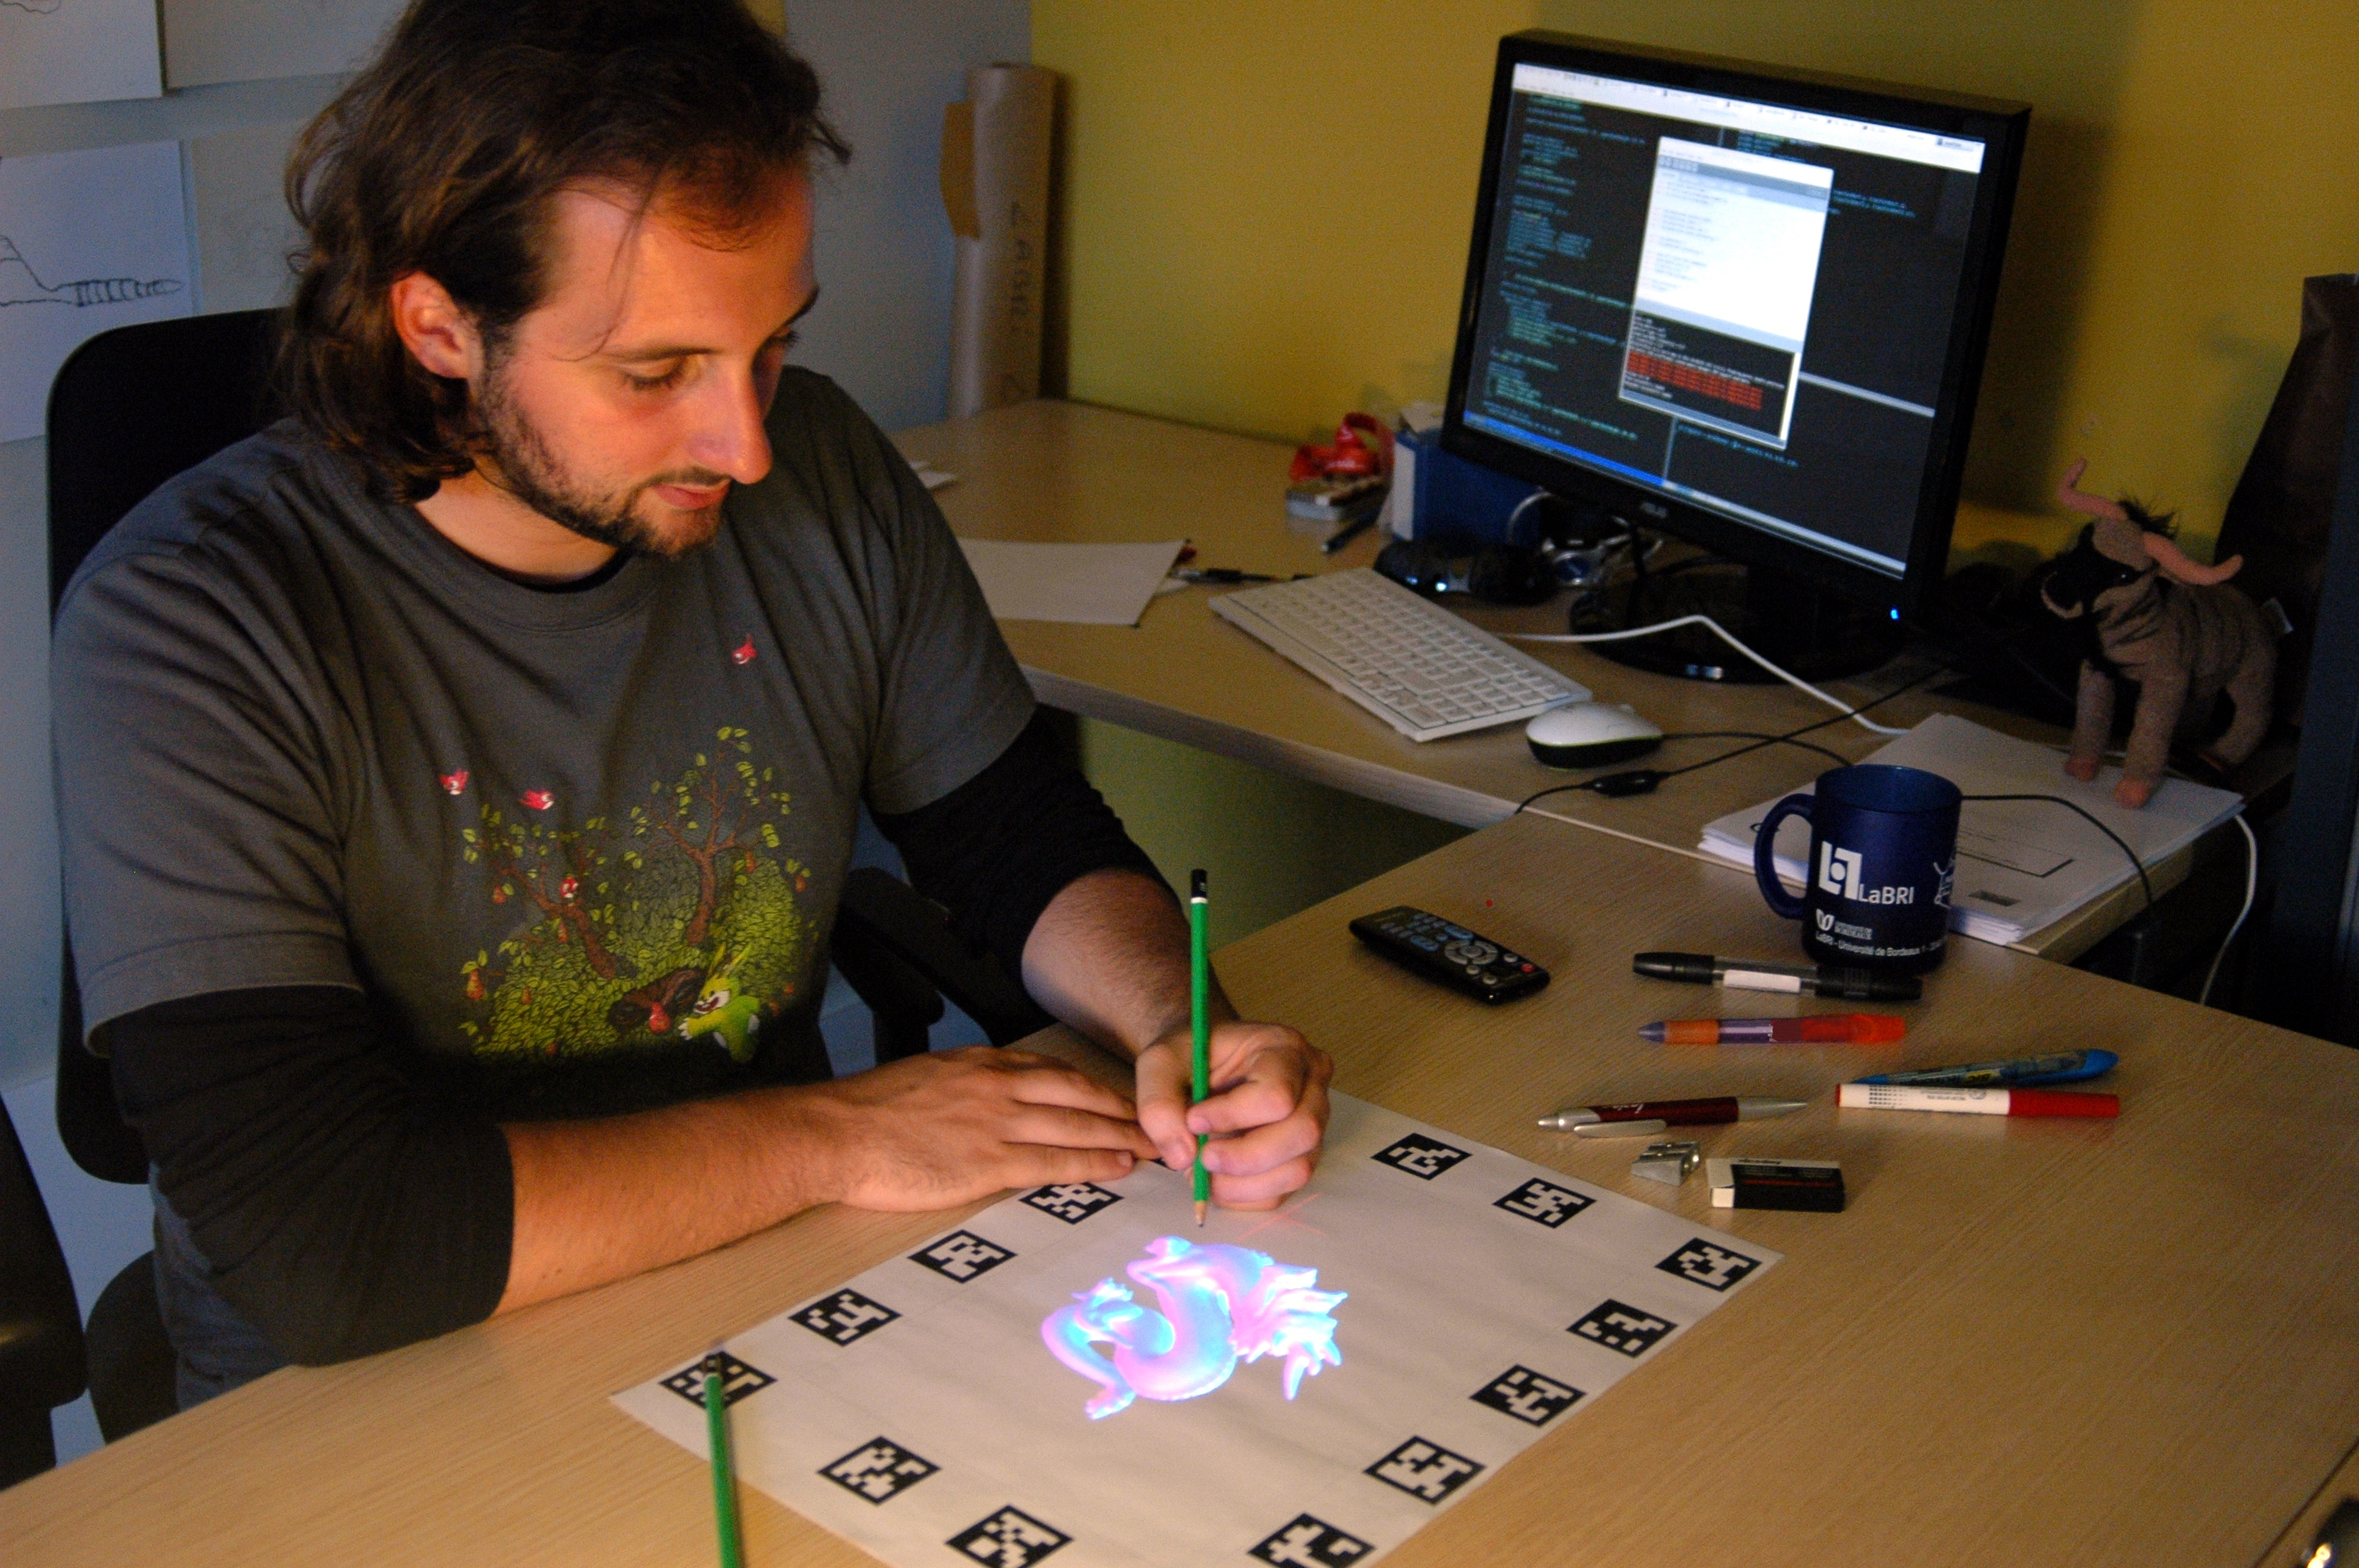
\includegraphics[width=0.65\textwidth]{images/papart-demo}
\caption{Jeremy Laviole utilisant \texttt{PapARt} pour dessiner en réalité augmentée\protect\footnotemark}
\label{fig:papartdemo}
\end{figure}
\footnotetext{Source: \href{https://team.inria.fr/potioc/fr/scientific-subjects_old/papart/}{Inria - \texttt{PapARt}}}

Le système interactif (fig~\ref{fig:papartsystem}) permettant d'utiliser tout le potentiel de \texttt{PapARt} est très spécifique et se compose de deux dispositifs d'acquisition.

Le premier est une caméra couleur observant la zone de travail. Son but est de détecter les feuilles de papier servant de base à la projection. Ces feuilles sont ornées de marqueurs ARToolKitPlus\footnote{\href{https://github.com/paroj/artoolkitplus}{https://github.com/paroj/artoolkitplus}}, une bibliothèque de détection de marqueurs fiduciaires \footnote{Un marqueur fiduciaire est un objet placé dans le champ de vision, le plus souvent d'un système d'imagerie, qui apparait sur l'image produite et qui va servir de point de repère ou de référence.}, qui ont deux utilisations. 
Dans un premier temps, ils permettent la détection de la feuille de papier. En effet, avec un nombre suffisant de marqueurs détectés et une connaissance à priori du modèle de la feuille, il est possible d'en estimer la pose \footnote{\href{https://en.wikipedia.org/wiki/Pose_(computer_vision)}{Pose : Wikipédia}} (position et rotation dans l'espace). 
Ces marqueurs servent également à identifier la feuille pour potentiellement en déterminer le contenu. Chaque marqueur étant unique, lorsque \texttt{PapARt} détecte une feuille de papier, il est également possible de récupérer les informations des marqueurs associés permettant de projeter du contenu différent en fonction des marqueurs présents.

Le deuxième dispositif d'acquisition est une caméra de profondeur dont le rôle est de détecter les différents utilisateurs, les différents objets et les potentielles interactions. Grâce aux informations de profondeur, les interactions peuvent être détectées soit sur le plan de la zone de travail, ce sont des interactions qualifiées de "touch", soit dans l'espace au dessus de la zone de travail, que l'on qualifiera de "pointage 3D".

Pour finir, en plus des deux dispositifs d'acquisition, un dispositif de projection est présent pour permettre la visualisation du contenu. Son rôle est de projeter, dans les zones adéquates (i.e détectées via des feuilles de marqueur), le contenu numérique désiré.

Pour que le projecteur soit capable de projeter précisément des informations sur les feuilles détectées par la caméra, une calibration très précise ainsi qu'une représentation à l'échelle est nécessaire. C'est aussi cette calibration qui permet au système d'avoir des capacités d'interaction (toucher simple, toucher multiple, balayage et autre) sensiblement similaires à celle d'une tablette tactile (fig ~\ref{fig:papart:touch}).

\begin{figure}
\centering
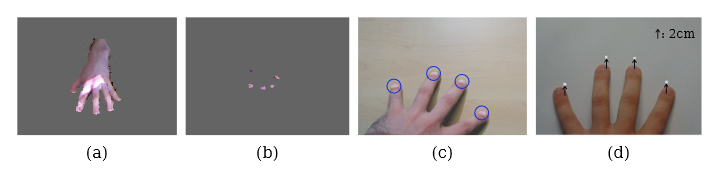
\includegraphics[width=\linewidth]{images/paparttouch}
\caption{ \texttt{PapARt} - Détection des interactions de "touch". (a) Détection de la main après opération de seuillage sur le plan de la table. (b) Sélection d'une zone de seulement 1-2cm au dessus de la table. (c) Projection sur les éléments détectés. (d) Décalage de la détection pour indiquer a l'utilisateur où l'interaction a été détectée.\protect\footnotemark}
\label{fig:papart:touch}
\end{figure}

\footnotetext{Source: \href{http://ori-oai.u-bordeaux1.fr/pdf/2013/LAVIOLE_JEREMY_2013.pdf}{Interaction en Réalité Augmentée Spatiale pour le Dessin Physique} - 2.3 SAR Système Multi-touch with Kinect}

\begin{figure}[H]
\centering
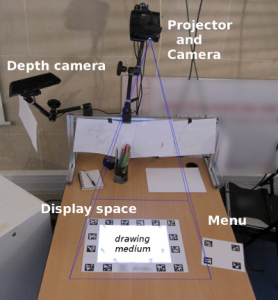
\includegraphics[width=0.4\textwidth]{images/papart-system}
\caption{Système interactif utilisant \texttt{PapARt}\protect\footnotemark}
\label{fig:papartsystem}
\end{figure}

\footnotetext{Source: \href{https://team.inria.fr/potioc/fr/scientific-subjects_old/papart/}{Inria - \texttt{PapARt}}}

Au-delà des applications d'aide au dessin qui sont aujourd'hui extrêmement nombreuses,\texttt{PapARt} laisse entrevoir une multitude de possibilités. Ainsi, l'objectif de RealityTech est d'explorer ce champ des possibles en améliorant \texttt{PapARt} et en présentant de nouveaux cas d'utilisation toujours plus innovants. Par exemple, RealityTech a récemment développé un système interactif permettant de vulgariser le fonctionnement d'un réseau de neurones Figure~\ref{fig:neuralnetwork}.

\begin{figure}[H]
\centering
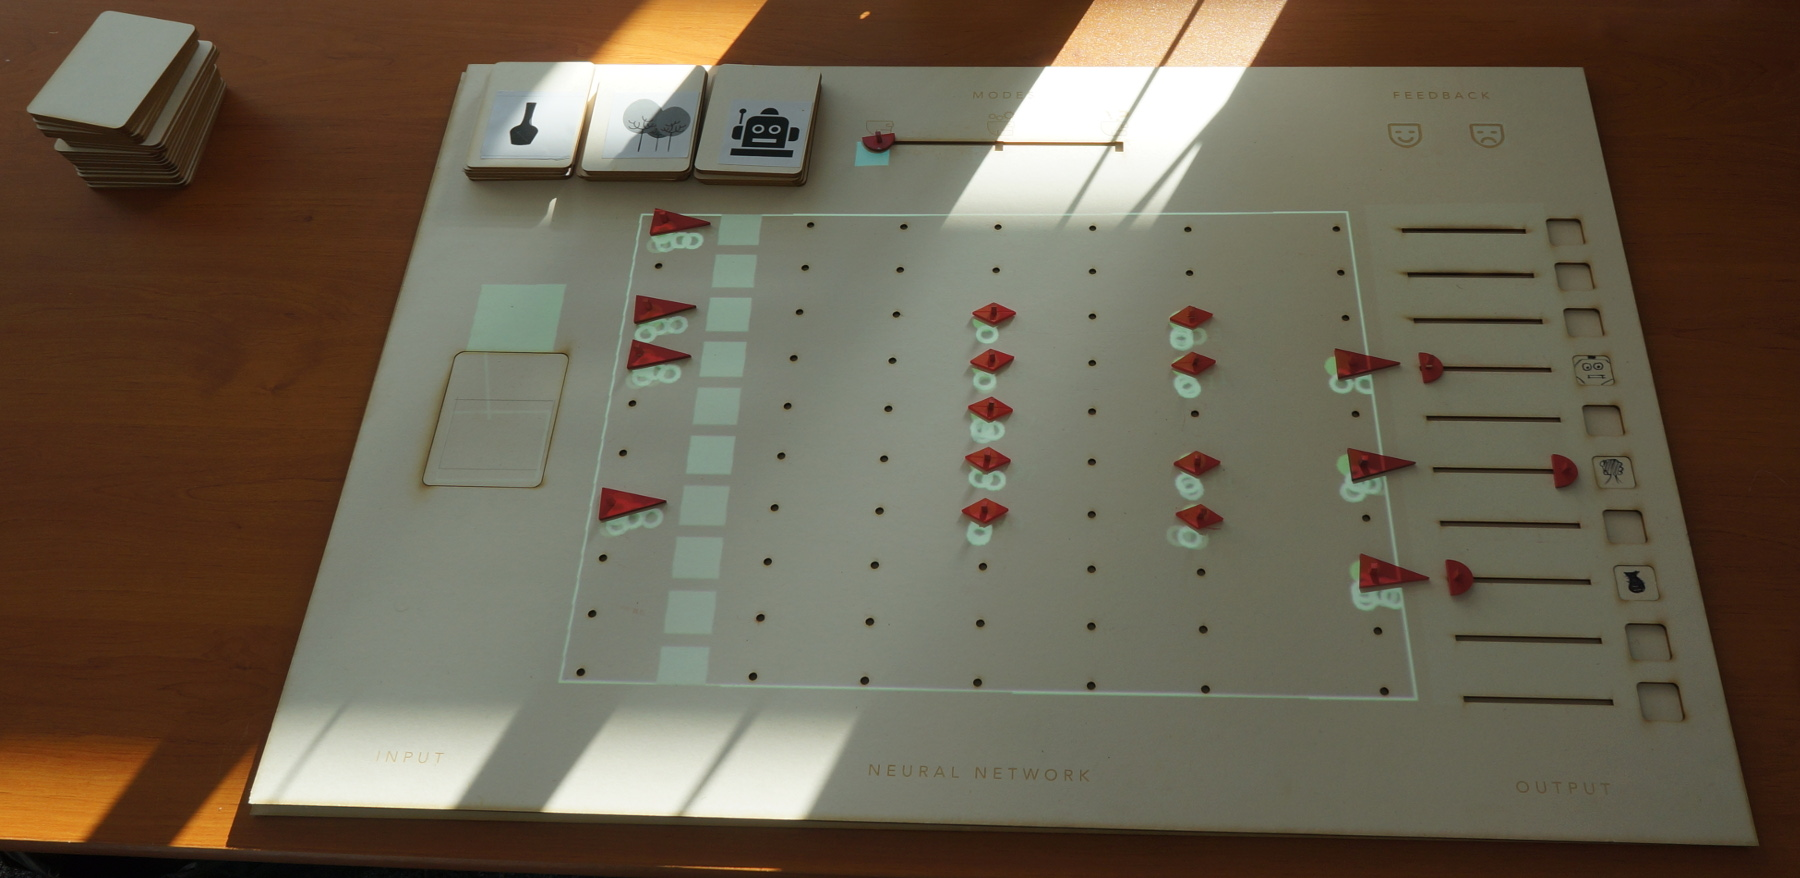
\includegraphics[width=0.65\linewidth]{images/neural-network}
\caption{Visualisation d'un réseau de neurone en réalité augmentée spatiale}
\label{fig:neuralnetwork}
\end{figure}


\section{Systèmes de réalité augmentée spatiale}
\label{sec:SARother}
\paragraph{RoomAliveToolKit} \texttt{RoomAliveToolKit}\cite{Jones:2014:RME:2642918.2647383} Figure~\ref{sub:roomalivesystem} est un projet tout droit sorti des laboratoires de recherche de Microsoft. Il s'agit d'un kit de développement créé en 2013 par Nikunj Raghuvanshi, Eyal Ofek et Andy Wilson qui permet, à l'instar de \texttt{\texttt{PapARt}}, de créer des expériences de projection interactive. La principale différence réside dans le fait que \texttt{RoomAliveToolKit} a pour but de donner vie à des pièces entières en utilisant plusieurs projecteurs et plusieurs caméra fonctionnant à l'unisson.

\texttt{RoomAliveToolKit} a permis, entre autres, de développer de nombreux projets basés sur de la projection interactive tels que \texttt{RoomAlive} Figure~\ref{sub:roomalivedemo}, \texttt{Room2Room}, ou encore \texttt{IllumiRoom} pour ne citer qu'eux.

\begin{figure}[H]
    \centering
	\subfloat[Système de projection interactive nécessaire à l'utilisation de \texttt{RoomAliveToolkit}]{
      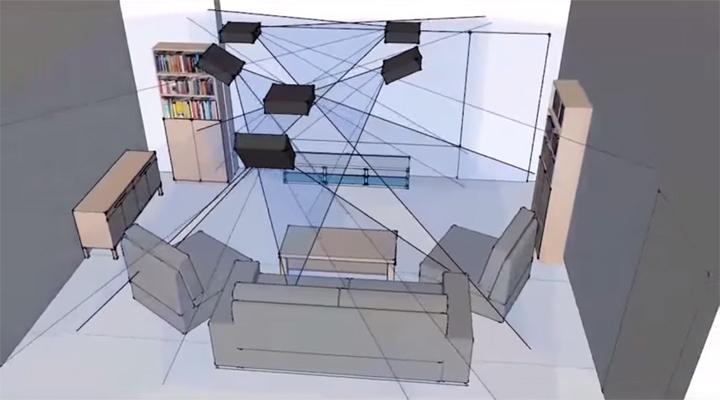
\includegraphics[width=0.45\textwidth]{images/roomalivesystem}
      \label{sub:roomalivesystem}
      }
    \subfloat[\texttt{RoomAlive} - Démonstration]{
      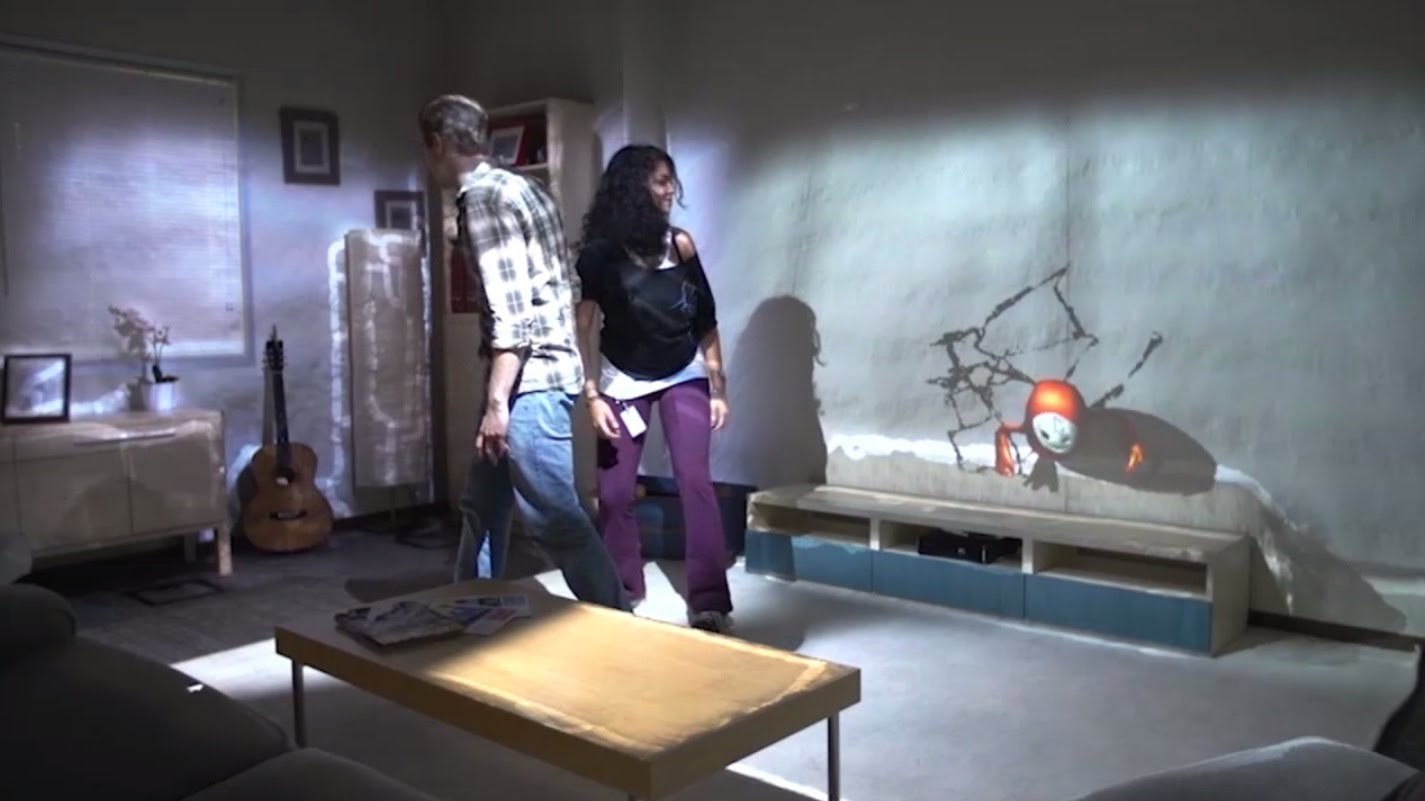
\includegraphics[width=0.45\textwidth]{images/roomalivedemo}
      \label{sub:roomalivedemo}
      }
\caption{Microsoft Research: \texttt{RoomAliveToolkit} et \texttt{RoomAlive}\protect\footnotemark}
\label{fig:roomalive}
\end{figure}
\footnotetext{Source: \href{https://github.com/Microsoft/RoomAliveToolkit}{RoomAliveToolkit}}

\paragraph{Lampix} Développé par Goerge Popescu et Mihai Dumitrescu, \texttt{Lampix} est un système de projection interactive dont le but est de rendre n'importe quelle surface horizontale "intelligente" (fig ~\ref{fig:lampix}). Le fonctionnement aussi bien logiciel que matériel de \texttt{Lampix} est très similaire à celui de \texttt{\texttt{PapARt}}. \texttt{Lampix} utilise de l'apprentissage et des techniques de vision par ordinateur pour proposer ces expériences. Étant donné que \texttt{Lampix} fonctionne via apprentissage, pour que le système fonctionne correctement et puisse évoluer, les créateurs de \texttt{Lampix} ont aussi créé la toute première blockchain\footnote{\href{https://fr.wikipedia.org/wiki/Blockchain}{Wikipédia: Blockchain}} dédiée à la vision par ordinateur contenant d'énormes jeux de données d'image labellisées (image et description).
     
\begin{figure}[H]
\centering
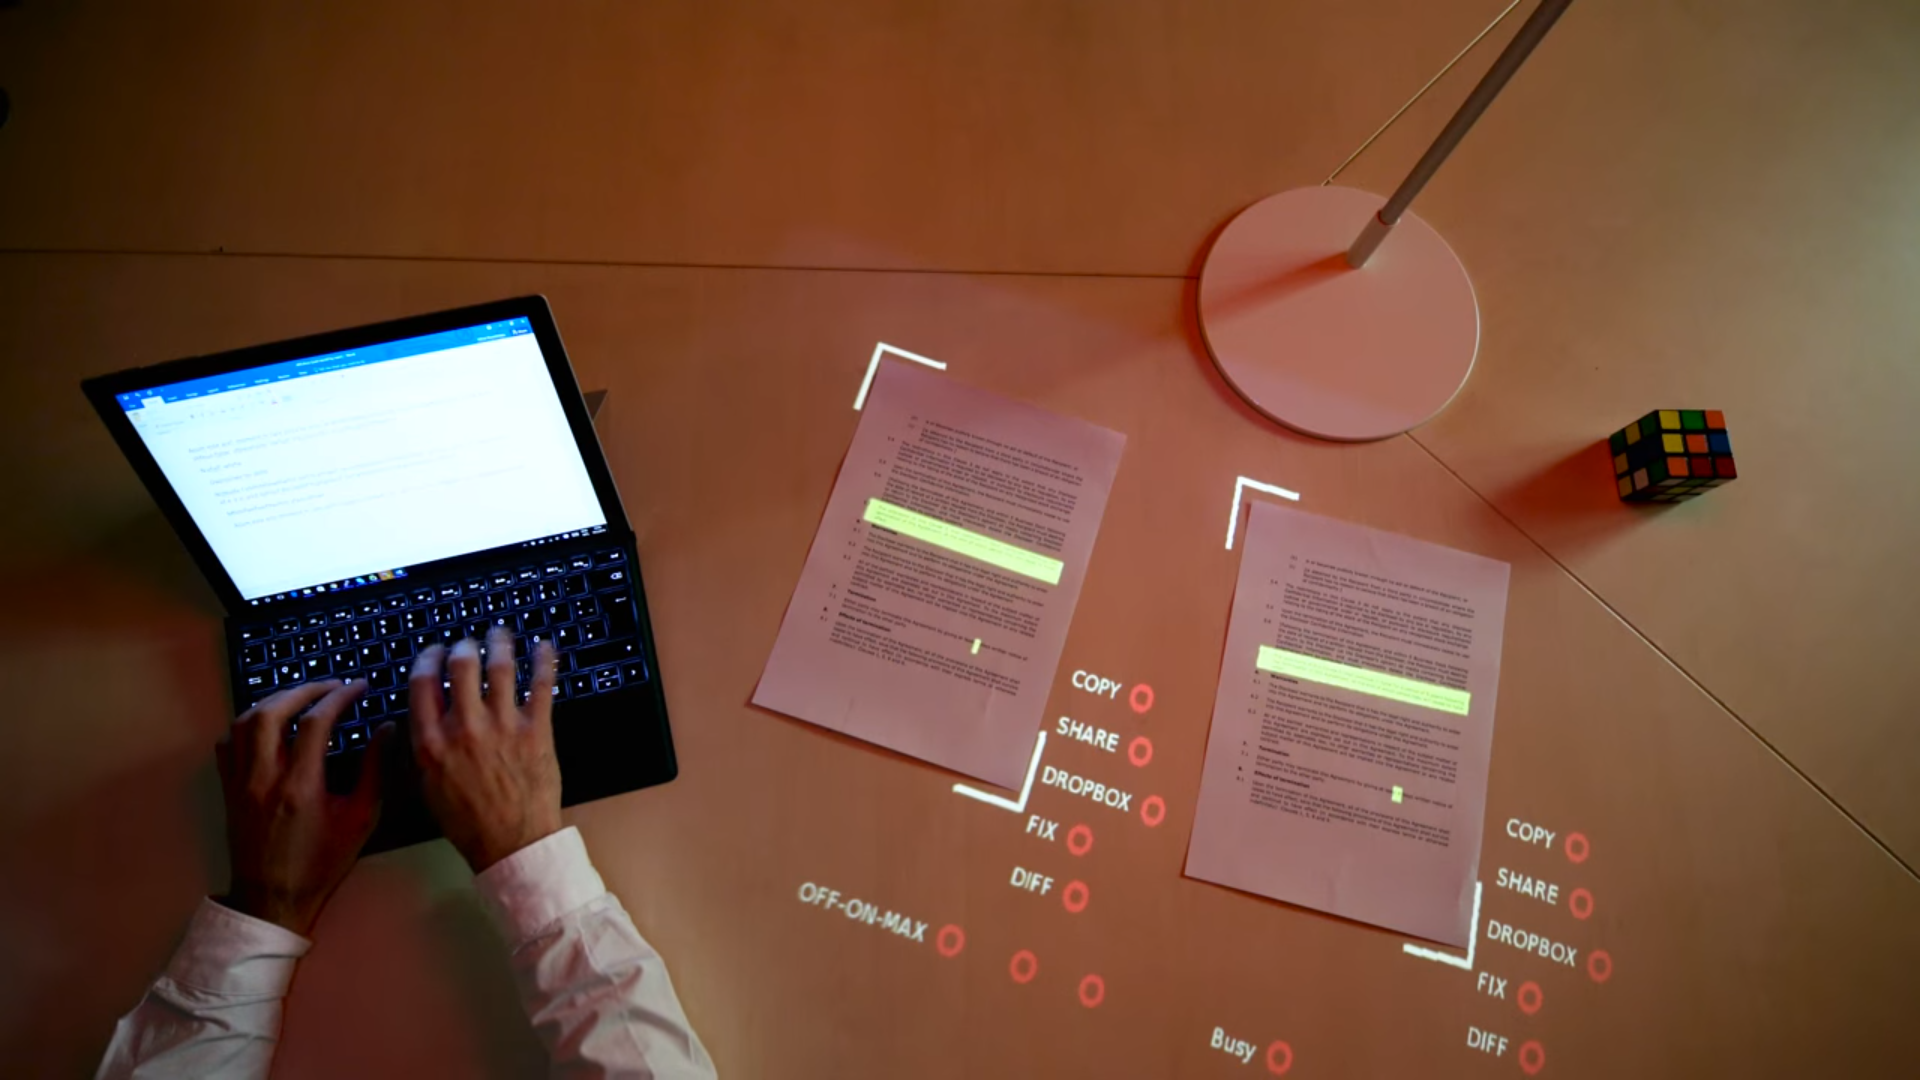
\includegraphics[width=0.7\linewidth]{images/lampix}
\caption{\texttt{Lampix} - Tabletop Augmented Reality Platform}
\label{fig:lampix}
\end{figure} 